\documentclass{beamer}

\pdfmapfile{+sansmathaccent.map}


\mode<presentation>
{
	\usetheme{Warsaw} % or try Darmstadt, Madrid, Warsaw, Rochester, CambridgeUS, ...
	\usecolortheme{seahorse} % or try seahorse, beaver, crane, wolverine, ...
	\usefonttheme{serif}  % or try serif, structurebold, ...
	\setbeamertemplate{navigation symbols}{}
	\setbeamertemplate{caption}[numbered]
} 


%%%%%%%%%%%%%%%%%%%%%%%%%%%%
% itemize settings


%%%%%%%%%%%%%%%%%%%%%%%%%%%%
% itemize settings

\definecolor{myhotpink}{RGB}{255, 80, 200}
\definecolor{mywarmpink}{RGB}{255, 60, 160}
\definecolor{mylightpink}{RGB}{255, 80, 200}
\definecolor{mypink}{RGB}{255, 30, 80}
\definecolor{mydarkpink}{RGB}{155, 25, 60}

\definecolor{mypaleblue}{RGB}{240, 240, 255}
\definecolor{mylightblue}{RGB}{120, 150, 255}
\definecolor{myblue}{RGB}{90, 90, 255}
\definecolor{mygblue}{RGB}{70, 110, 240}
\definecolor{mydarkblue}{RGB}{0, 0, 180}
\definecolor{myblackblue}{RGB}{40, 40, 120}

\definecolor{mygreen}{RGB}{0, 200, 0}
\definecolor{mygreen2}{RGB}{245, 255, 230}

\definecolor{mygray}{gray}{0.8}
\definecolor{mydarkgray}{RGB}{80, 80, 160}

\definecolor{mydarkred}{RGB}{160, 30, 30}
\definecolor{mylightred}{RGB}{255, 150, 150}
\definecolor{myred}{RGB}{200, 110, 110}
\definecolor{myblackred}{RGB}{120, 40, 40}

\definecolor{mygreen}{RGB}{0, 200, 0}
\definecolor{mygreen2}{RGB}{205, 255, 200}

\definecolor{mydarkcolor}{RGB}{60, 25, 155}
\definecolor{mylightcolor}{RGB}{130, 180, 250}

\setbeamertemplate{itemize items}[default]

\setbeamertemplate{itemize item}{\color{myblackblue}$\blacksquare$}
\setbeamertemplate{itemize subitem}{\color{mygblue}$\blacktriangleright$}
\setbeamertemplate{itemize subsubitem}{\color{mygray}$\blacksquare$}

\setbeamercolor{palette quaternary}{fg=white,bg=mydarkgray}
\setbeamercolor{titlelike}{parent=palette quaternary}

\setbeamercolor{palette quaternary2}{fg=black,bg=mypaleblue}
\setbeamercolor{frametitle}{parent=palette quaternary2}

\setbeamerfont{frametitle}{size=\Large,series=\scshape}
\setbeamerfont{framesubtitle}{size=\normalsize,series=\upshape}





%%%%%%%%%%%%%%%%%%%%%%%%%%%%
% block settings

\setbeamercolor{block title}{bg=red!30,fg=black}

\setbeamercolor*{block title example}{bg=mygreen!40!white,fg=black}

\setbeamercolor*{block body example}{fg= black, bg= mygreen2}


%%%%%%%%%%%%%%%%%%%%%%%%%%%%
% URL settings
\hypersetup{
	colorlinks=true,
	linkcolor=blue,
	filecolor=blue,      
	urlcolor=blue,
}

%%%%%%%%%%%%%%%%%%%%%%%%%%

\renewcommand{\familydefault}{\rmdefault}

\usepackage{amsmath}
\usepackage{mathtools}

\usepackage{subcaption}

\usepackage{qrcode}

\DeclareMathOperator*{\argmin}{arg\,min}
\newcommand{\bo}[1] {\mathbf{#1}}

\newcommand{\R}{\mathbb{R}} 
\newcommand{\T}{^\top}     

\newcommand{\dx}[1] {\dot{\mathbf{#1}}}
\newcommand{\ma}[4] {\begin{bmatrix}
		#1 & #2 \\ #3 & #4
\end{bmatrix}}
\newcommand{\myvec}[2] {\begin{bmatrix}
		#1 \\ #2
\end{bmatrix}}
\newcommand{\myvecT}[2] {\begin{bmatrix}
		#1 & #2
\end{bmatrix}}


\newcommand{\mydate}{Spring 2023}

\newcommand{\mygit}{\textcolor{blue}{\href{https://github.com/SergeiSa/Control-Theory-Slides-Spring-2023}{github.com/SergeiSa/Control-Theory-Slides-Spring-2023}}}

\newcommand{\myqr}{ \textcolor{black}{\qrcode[height=1.5in]{https://github.com/SergeiSa/Control-Theory-Slides-Spring-2023}}
}

\newcommand{\myqrframe}{
	\begin{frame}
		\centerline{Lecture slides are available via Github, links are on Moodle}
		\bigskip
		\centerline{You can help improve these slides at:}
		\centerline{\mygit}
		\bigskip
		\myqr
	\end{frame}
}


\newcommand{\bref}[2] {\textcolor{blue}{\href{#1}{#2}}}

%%%%%%%%%%%%%%%%%%%%%%%%%%%%
% code settings

\usepackage{listings}
\usepackage{color}
% \definecolor{mygreen}{rgb}{0,0.6,0}
% \definecolor{mygray}{rgb}{0.5,0.5,0.5}
\definecolor{mymauve}{rgb}{0.58,0,0.82}
\lstset{ 
	backgroundcolor=\color{white},   % choose the background color; you must add \usepackage{color} or \usepackage{xcolor}; should come as last argument
	basicstyle=\footnotesize,        % the size of the fonts that are used for the code
	breakatwhitespace=false,         % sets if automatic breaks should only happen at whitespace
	breaklines=true,                 % sets automatic line breaking
	captionpos=b,                    % sets the caption-position to bottom
	commentstyle=\color{mygreen},    % comment style
	deletekeywords={...},            % if you want to delete keywords from the given language
	escapeinside={\%*}{*)},          % if you want to add LaTeX within your code
	extendedchars=true,              % lets you use non-ASCII characters; for 8-bits encodings only, does not work with UTF-8
	firstnumber=0000,                % start line enumeration with line 0000
	frame=single,	                   % adds a frame around the code
	keepspaces=true,                 % keeps spaces in text, useful for keeping indentation of code (possibly needs columns=flexible)
	keywordstyle=\color{blue},       % keyword style
	language=Octave,                 % the language of the code
	morekeywords={*,...},            % if you want to add more keywords to the set
	numbers=left,                    % where to put the line-numbers; possible values are (none, left, right)
	numbersep=5pt,                   % how far the line-numbers are from the code
	numberstyle=\tiny\color{mygray}, % the style that is used for the line-numbers
	rulecolor=\color{black},         % if not set, the frame-color may be changed on line-breaks within not-black text (e.g. comments (green here))
	showspaces=false,                % show spaces everywhere adding particular underscores; it overrides 'showstringspaces'
	showstringspaces=false,          % underline spaces within strings only
	showtabs=false,                  % show tabs within strings adding particular underscores
	stepnumber=2,                    % the step between two line-numbers. If it's 1, each line will be numbered
	stringstyle=\color{mymauve},     % string literal style
	tabsize=2,	                   % sets default tabsize to 2 spaces
	title=\lstname                   % show the filename of files included with \lstinputlisting; also try caption instead of title
}


%%%%%%%%%%%%%%%%%%%%%%%%%%%%
% URL settings
\hypersetup{
	colorlinks=false,
	linkcolor=blue,
	filecolor=blue,      
	urlcolor=blue,
}

%%%%%%%%%%%%%%%%%%%%%%%%%%

%%%%%%%%%%%%%%%%%%%%%%%%%%%%
% tikz settings

\usepackage{tikz}
\tikzset{every picture/.style={line width=0.75pt}}


\title{Stability}
\subtitle{Control Theory, Lecture 2}
\author{by Sergei Savin}
\centering
\date{\mydate}



\begin{document}
\maketitle


\begin{frame}{Content}

\begin{itemize}
\item Critical point (node)
\item Stability
\item Asymptotic stability
\item Stability vs Asymptotic stability
\item LTI and autonomous LTI
\item Stability of autonomous LTI
\item Read more
\end{itemize}

\end{frame}



\begin{frame}{Critical point (node)}
% \framesubtitle{O}
\begin{flushleft}

Consider the following ODE:

\begin{equation}
    \dot{\bo{x}} = \bo{f} (\bo{x}, t)
\end{equation}

Let $\bo{x}_0$ be such a state that:

\begin{equation}
    \bo{f} (\bo{x}_0, t) = 0
\end{equation}

Then such state $\bo{x}_0$ is called a \emph{node} or a \emph{critical point}.

\end{flushleft}
\end{frame}



\begin{frame}{Stability}
% \framesubtitle{O}
\begin{flushleft}

Node $\bo{x}_0$ is called \emph{stable} iff for any constant $\delta$ there exists constant $\varepsilon$ such that:

\begin{equation}
    ||\bo{x}(0) - \bo{x}_0|| < \delta \ \longrightarrow \ ||\bo{x}(t) - \bo{x}_0|| < \varepsilon
\end{equation}

\bigskip

Think of it as "for any initial point that lies at most $\delta$ away from $\bo{x}_0$, the rest of the trajectory $\bo{x}(t)$ will be at most $\varepsilon$ away from $\bo{x}_0$".

\bigskip

Or, more picturesque, think of it as "the solutions starting from $\delta$-sized ball do not diverge"

\end{flushleft}
\end{frame}


\begin{frame}{Asymptotic stability}
% \framesubtitle{O}
\begin{flushleft}

Node $\bo{x}_0$ is called \emph{asymptotically stable} iff for any constant $\delta$ it is true that:

\begin{equation}
    ||\bo{x}(0) - \bo{x}_0|| < \delta \ \longrightarrow \ 
    \lim_{t\to\infty} \bo{x}(t) = \bo{x}_0
\end{equation}

\bigskip

Think of it as "for any initial point that lies at most $\delta$ away from $\bo{x}_0$, the trajectory $\bo{x}(t)$ will asymptotically approach the point $\bo{x}_0$".

\bigskip

Or, more picturesque, think of it as ""the solutions starting from $\delta$-sized ball converge to the node"

\end{flushleft}
\end{frame}




\begin{frame}{Stability vs Asymptotic stability}
% \framesubtitle{O}
\begin{flushleft}

\begin{example}
Consider dynamical system $\dot{x} = 0$, and solution $x = 7$. This solution is stable, but not asymptotically stable (other solutions do not diverge from $x = 7$, but do not converge to it either).
\end{example}

\begin{example}
Consider dynamical system $\dot{x} = -x$, and solution $x = 0$. This solution is stable and asymptotically stable (other solutions converge to $x = 0$).
\end{example}

\begin{example}
Consider dynamical system $\dot{x} = x$, and solution $x = 0$. This solution is unstable (other solutions diverge from $x = 0$).
\end{example}

\end{flushleft}
\end{frame}



\begin{frame}{Linear systems}
% \framesubtitle{O}
\begin{flushleft}

Consider the following linear ODE:

\begin{equation}
    \dot{\bo{x}} = \bo{A} \bo{x} + \bo{B} \bo{u}
\end{equation}

This is called a \emph{linear time-invariant system}, or \emph{LTI}, indicating that $\bo{A}$ and $\bo{B}$ are constant.

\bigskip

Removing the input we find an even simpler equation:

\begin{equation}
    \dot{\bo{x}} = \bo{A} \bo{x}
\end{equation}

This is also an LTI, and it is also called an \emph{autonomous system}, since its evolution depends only on the state of the system.

\end{flushleft}
\end{frame}




\begin{frame}{Stability of autonomous LTI}
	\framesubtitle{Real eigenvalues}
	\begin{flushleft}
		
		Consider autonomous LTI:
		
		\begin{equation}
			\dot{\bo{x}} = \bo{D} \bo{x}
		\end{equation}
		
		where $\bo{D} = \text{diag}(d_1, \ ..., \ d_n)$ is a diagonal matrix. This is the same as a system of independent equations: 
		
		\begin{equation}
			\begin{cases}
				\dot{x}_1 = d_1 x_1 \\
				... \\
				\dot{x}_n = d_n x_n
			\end{cases}
		\end{equation}		
		
		Each of these equations has an exact solution $ x_i = C_i e^{d_i t}$. It diverges from 0 if $d_i > 0$, it does not diverge if $d_i \leq 0$ and it converges to 0 if $d_i < 0$.
		
	\end{flushleft}
\end{frame}


\begin{frame}{Stability of autonomous LTI}
\framesubtitle{Real eigenvalues}
\begin{flushleft}

Consider autonomous LTI:

\begin{equation}
    \dot{\bo{x}} = \bo{A} \bo{x}
\end{equation}

where $\bo{A}$ can be decomposed via eigen-decomposition as $\bo{A} = \bo{V} \bo{D} \bo{V}^{-1}$, where $\bo{D}$ is a diagonal matrix. 

\bigskip

\begin{equation}
    \dot{\bo{x}} = \bo{V} \bo{D} \bo{V}^{-1} \bo{x}
\end{equation}

Multiplying it by $\bo{V}^{-1}$ 
we get: 
$\bo{V}^{-1} \dot{\bo{x}} = \bo{V}^{-1} \bo{V} \bo{D} \bo{V}^{-1} \bo{x}$.

Defining $\bo{z} = \bo{V}^{-1} \bo{x}$ we transform the equation: 
$\dot{\bo{z}} = \bo{D} \bo{z}$.

\bigskip

Since elements of $\bo{D}$ are real, we can clearly see, that iff they are \emph{all negative} will the system be asymptotically stable. If they are non-positive, the system is stable. And those elements are eigenvalues of $\bo{A}$.

\end{flushleft}
\end{frame}




\begin{frame}{Upper triangular matrices}
%	\framesubtitle{Real eigenvalues}
	\begin{flushleft}
		
		Examples of upper triangular matrices are:
		
		\begin{equation}
			\begin{bmatrix}
				1 & 5 & -2 \\
				0 & 3 & 1 \\
				0 & 0 & -2
			\end{bmatrix},
		\ \ \ 
		\begin{bmatrix}
			-2 & 0 & 8 \\
			0 & -2 & 8 \\
			0 & 0 & 7
		\end{bmatrix},
	\ \ \ 
		\begin{bmatrix}
			4 & 1 \\
			0 & 3
		\end{bmatrix}
		\end{equation}
		
		Eigenvalues of upper triangular matrices are the diagonal elements of these matrices.
		
	\end{flushleft}
\end{frame}


\begin{frame}{Upper triangular matrices}
	%	\framesubtitle{Real eigenvalues}
	\begin{flushleft}
		
		Consider autonomous LTI:
		
		\begin{equation}
			\dot{\bo{x}} = \bo{M} \bo{x}
		\end{equation}
	
	where $ \bo{M}$ is an upper triangular matrices with negative eigenvalues $m_{1,1}$, ... $m_{n,n}$.
	
	\bigskip
	
	The last equation is $\dot x_n = m_{n,n} x_n$, and since $m_{n,n} < 0$ we can observe that $\underset{t \rightarrow \infty}{\text{lim}} x_n(t) = 0$.
	
	\bigskip
	
	The equation \# n-1 is $\dot x_{n-1} = m_{n-1,n-1} x_{n-1} + m_{n-1,n} x_n$, and since $m_{n-1,n-1} < 0$ and $\underset{t \rightarrow \infty}{\text{lim}} x_n(t) = 0$ we can observe that $\underset{t \rightarrow \infty}{\text{lim}} x_{n-1}(t) = 0$.
	
	This can be repeated for all equations, proving asymptotic stability for the system.
	
	\end{flushleft}
\end{frame}




\begin{frame}{Stability of autonomous LTI}
\framesubtitle{Complex eigenvalues, 2-dimensional case (1)}
\begin{flushleft}

Let us consider the following system:

\begin{equation}
\begin{bmatrix}
    \dot{\bo{x}}_1 \\ \dot{\bo{x}}_2
\end{bmatrix}
     = 
\begin{bmatrix}
    \alpha & -\beta \\ \beta & \alpha
\end{bmatrix}     
\begin{bmatrix}
    \bo{x}_1 \\ \bo{x}_2
\end{bmatrix}
\end{equation}

The eigenvalues of the system are $\alpha \pm i \beta$. We denote $\begin{bmatrix}
    \bo{x}_1 \\ \bo{x}_2
\end{bmatrix} = \bo{x}$.

\bigskip

We start by claiming that the system will be stable iff the $\dot{\bo{x}}^\top \bo{x} < 0$. Indeed, vector $\dot{\bo{x}}$ can always be decomposed into two components, $\dot{\bo{x}}_{||}$ parallel to $\bo{x}$, and $\dot{\bo{x}}_{\perp}$ perpendicular to $\bo{x}$. By definition $\dot{\bo{x}}_{\perp}^\top \bo{x} = 0$, and is responsible for the change in orientation of $\bo{x}$. The value of $\dot{\bo{x}}_{||}$ is responsible for the change in the length of $\bo{x}$; the length would shrink iff $\dot{\bo{x}}_{||}$ is of opposite direction to $\bo{x}$, giving negative value of the dot product $\dot{\bo{x}}^\top \bo{x}$.

\end{flushleft}
\end{frame}



\begin{frame}{Stability of autonomous LTI}
\framesubtitle{Complex eigenvalues, 2-dimensional case (2)}
\begin{flushleft}

Let us compute $\dot{\bo{x}}^\top \bo{x}$:

\begin{equation}
\dot{\bo{x}}^\top \bo{x} =
\begin{bmatrix}
    \bo{x}_1 & \bo{x}_2
\end{bmatrix}
\begin{bmatrix}
    \alpha & -\beta \\ \beta & \alpha
\end{bmatrix}     
\begin{bmatrix}
    \bo{x}_1 \\ \bo{x}_2
\end{bmatrix}
\end{equation}

\begin{equation}
\dot{\bo{x}}^\top \bo{x} =
\alpha (\bo{x}_1^2 + \bo{x}_2^2)
\end{equation}

From this it is clear that the product $\dot{\bo{x}}^\top \bo{x} < 0$ is negative iff $\alpha < 0$.

\begin{definition}
As long as the \emph{real parts of the eigenvalues} of the system are \emph{strictly negative}, the system is \emph{asymptotically stable}. If the real parts of the eigenvalues of the system are zero, the system is \emph{marginally stable}.
\end{definition}

\end{flushleft}
\end{frame}



\begin{frame}{Stability of autonomous LTI}
\framesubtitle{Complex eigenvalues, 2-dimensional case (3)}
\begin{flushleft}

Vector field of 
$\begin{bmatrix}
    \dot{\bo{x}}_1 \\ \dot{\bo{x}}_2
\end{bmatrix} 
=
\begin{bmatrix}
    \alpha & -\beta \\ \beta & \alpha
\end{bmatrix}     
\begin{bmatrix}
    \bo{x}_1 \\ \bo{x}_2
\end{bmatrix} $ 
is shown below:
%
\begin{figure}
    \centering
    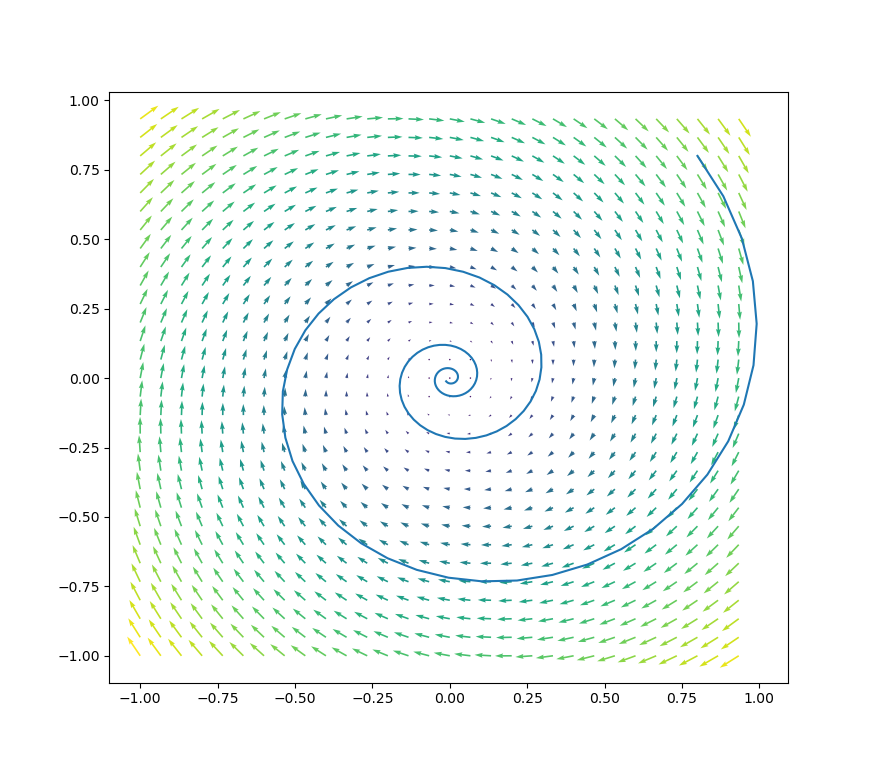
\includegraphics[width=7cm]{Figure_1.png}%, width=7cm
    % \caption{Caption}
    \label{fig:my_label}
\end{figure}

\end{flushleft}
\end{frame}



\begin{frame}{Stability of autonomous LTI}
\framesubtitle{General case (1)}
\begin{flushleft}

Given $\dot{\bo{x}} = \bo{A} \bo{x}$, where $\bo{A}$ can be decomposed via eigen-decomposition as $\bo{A} = \bo{U} \bo{C} \bo{U}^{-1}$, where $\bo{C}$ is a complex-valued diagonal matrix and $\bo{U}$ is a complex-valued inevitable matrix. 

\bigskip

We multiply both sides by $\bo{U}^{-1}$, then define $\bo{z} = \bo{U}^{-1} \bo{x}$ to arrive at:

\begin{equation}
    \dot{\bo{z}} = \bo{C} \bo{z}
\end{equation}

which falls into a set of independent equations, with complex coefficients $c_j$:

\begin{equation}
    \dot{z}_j = c_j z_j
\end{equation}

\end{flushleft}
\end{frame}



\begin{frame}{Stability of autonomous LTI}
\framesubtitle{General case (2)}
\begin{flushleft}

Expanding $c_j = \alpha + i \beta$, and $z_j = u + i v$ (we dismiss subscripts for clarity), we find that $\dot{z}_j = c_j z_j$ can be expanded as:

\begin{equation}
    \dot{u} + i \dot{v} = \dot{z}_j = c_j z_j = (\alpha + i \beta) (u + i v)
\end{equation}
%
\begin{equation}
    \dot{u} + i \dot{v} = \alpha u + i \beta u + i \alpha v - \beta v
\end{equation}
%
\begin{equation}
\begin{bmatrix}
    \dot{u} \\ \dot{v}
\end{bmatrix}
     = 
\begin{bmatrix}
    \alpha & -\beta \\ \beta & \alpha
\end{bmatrix}     
\begin{bmatrix}
    u \\ v
\end{bmatrix}
\end{equation}

As we can see, $\dot{z}_j = c_j z_j$ is asymptotically stable iff $\text{Re}(c_j) < 0$, and marginally stable if $\alpha = \text{Re}(c_j) = 0$. Same is true for $\dot{\bo{z}} = \bo{C} \bo{z}$ and hence, for $\dot{\bo{x}} = \bo{A} \bo{x}$, as $\bo{U}$ is invertible.

\end{flushleft}
\end{frame}




\begin{frame}{Stability of autonomous LTI}
\framesubtitle{Condition}
\begin{flushleft}

Consider an autonomous LTI:

\begin{equation}
\label{eq:LTI}
    \dot{\bo{x}} = \bo{A} \bo{x}
\end{equation}

\begin{definition}
Eq. \eqref{eq:LTI} is stable iff real parts of eigenvalues of $\bo{A}$ are non-positive.
\end{definition}

\begin{definition}
Eq. \eqref{eq:LTI} is asymptotically stable iff real parts of eigenvalues of $\bo{A}$ are negative.
\end{definition}

\end{flushleft}
\end{frame}




\begin{frame}{Stability of autonomous LTI}
\framesubtitle{Illustration}
\begin{flushleft}

Here is an illustration of \emph{phase portraits} of two-dimensional LTIs with different types of stability:

\begin{figure}
    \centering
    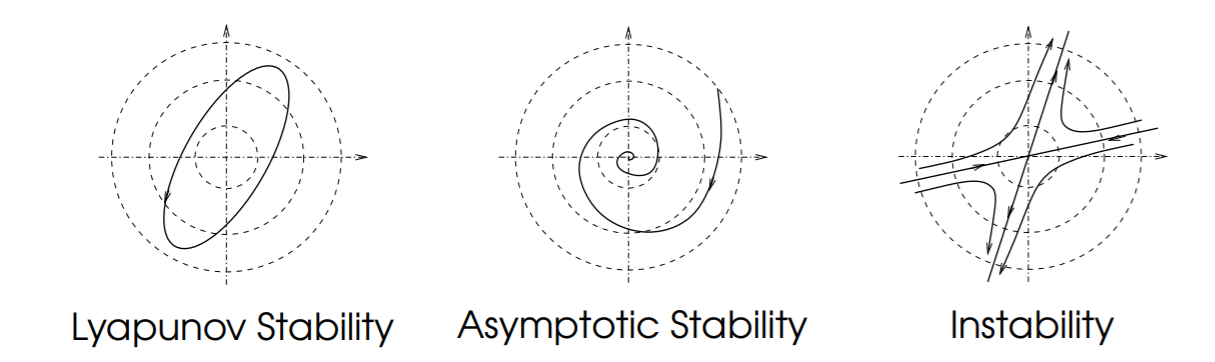
\includegraphics[width=1.0\linewidth]{Stability.PNG}
    \caption{phase portraits for different types of stability}
    \label{fig:Stability}
\end{figure}

\bigskip

\scriptsize{Credit: \bref{http://staff.uz.zgora.pl/wpaszke/materialy/spc/Lec13.pdf}{staff.uz.zgora.pl/wpaszke/materialy/spc/Lec13.pdf}}

\end{flushleft}
\end{frame}


\begin{frame}
\hspace*{-2.5cm}
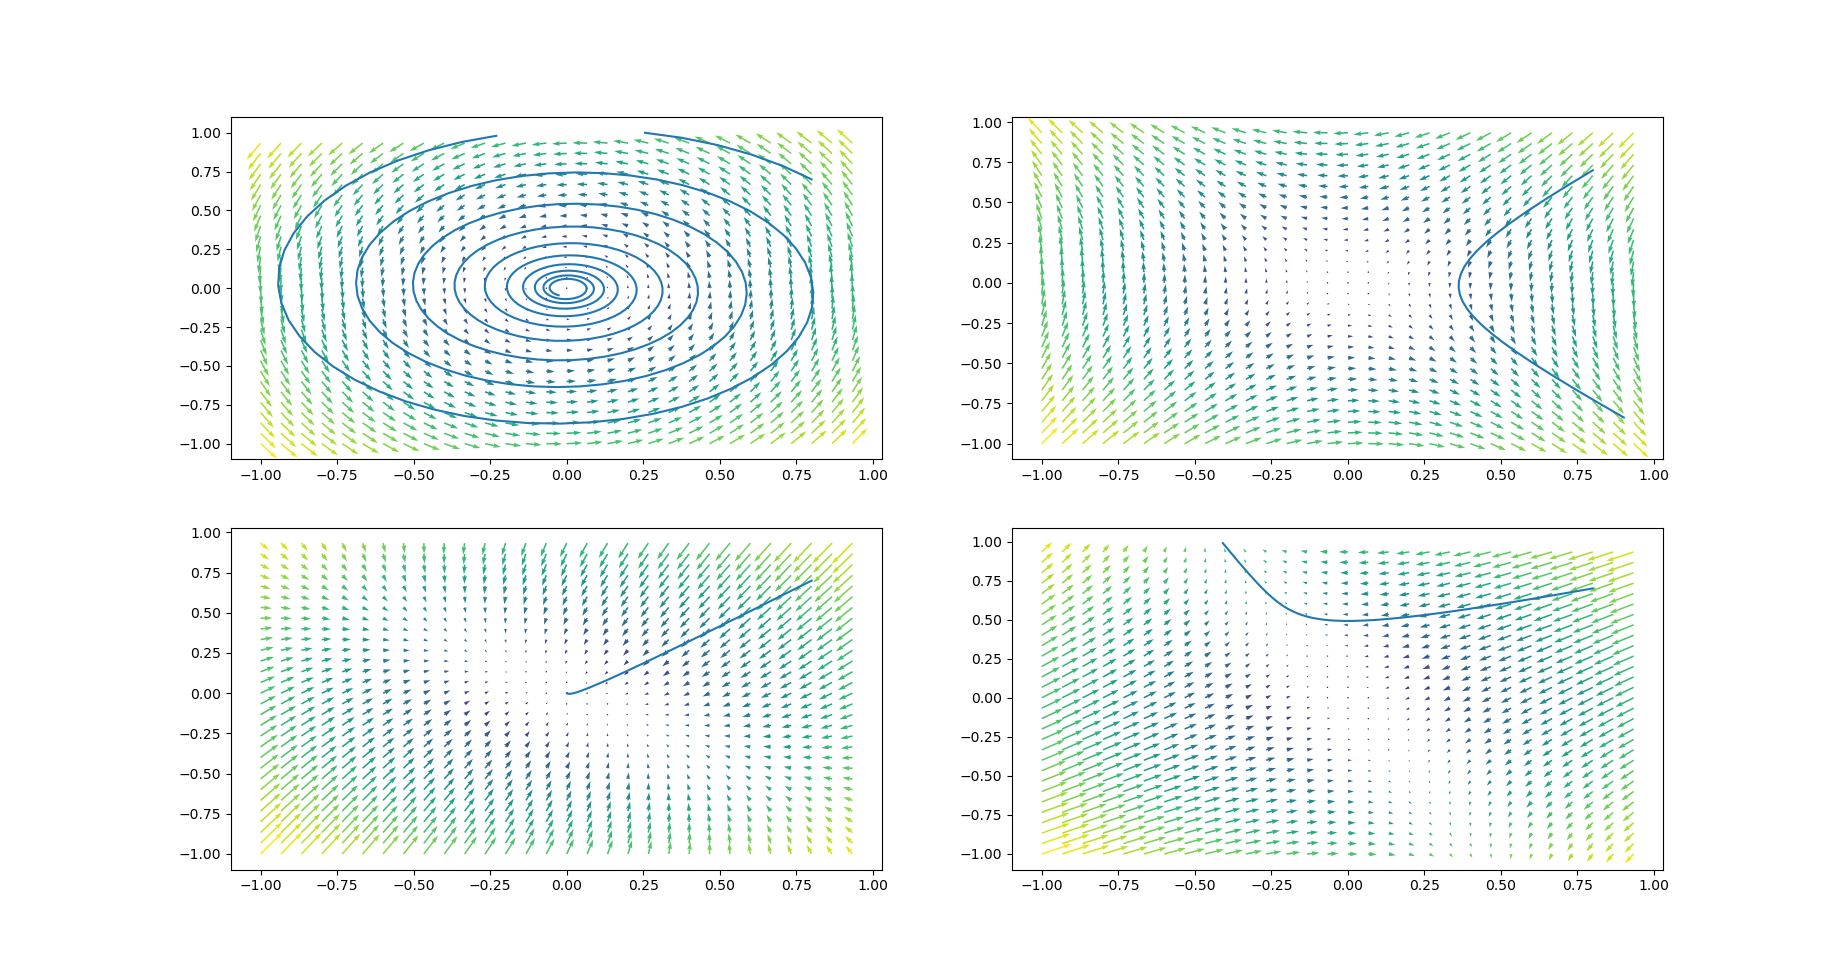
\includegraphics[height=\textheight,width=1.4\textwidth,keepaspectratio]{Figure_2.png}
\end{frame}



\begin{frame}{Read/Watch more}

\begin{itemize}
\item Control Systems Design, by Julio H. Braslavsky \bref{http://staff.uz.zgora.pl/wpaszke/materialy/spc/Lec13.pdf}{staff.uz.zgora.pl/wpaszke/materialy/spc/Lec13.pdf}

\item Stability and Eigenvalues, Steve Brunton \bref{https://youtu.be/h7nJ6ZL4Lf0 }{youtu.be/h7nJ6ZL4Lf0}

\item MAE509 (LMIs in Control): Lecture 4, part A - Stability and Eigenvalues  \bref{https://youtu.be/8zYOJbpiT38 }{youtu.be/8zYOJbpiT38}

\end{itemize}

\end{frame}



\begin{frame}{Thank you!}
\centerline{Lecture slides are available via Moodle.}
\bigskip
\centerline{You can help improve these slides at:}
\centerline{\mygit}
\bigskip
\centerline{Check Moodle for additional links, videos, textbook suggestions.}
\bigskip

\centerline{\textcolor{black}{\qrcode[height=1.6in]{https://github.com/SergeiSa/Control-Theory-Slides-Spring-2022}}}
\end{frame}

\end{document}
